
\documentclass[10pt, conference, compsocconf,a4paper]{IEEEtran}

\RequirePackage{nybohansenPreamble}

% correct bad hyphenation here
\hyphenation{op-tical net-works semi-conduc-tor}


\begin{document}
\title{Extending Mocapy++ with a mixed probability distribution\\Advanced Topics In Data Modeling}

\author{\IEEEauthorblockN{Kasper Nybo Hansen}
\IEEEauthorblockA{Dept. of Computer Science\\
University of Copenhagen\\
Copenhagen, Denmark\\
nybo@diku.dk}
}

% make the title area
\maketitle



\begin{abstract}
Mocapy++ is a C++ toolkit for learning and inference in dynamic Bayesian networks. This report describes the implementation, testing and results of extending Mocapy++ with a new node. 

The new node is a mixed node, allowing both discrete and continuous values. The continuous part of the node is a gaussian distribution. The new node is used to calculate a probabilistic model of hydrogen bonding in protein structures. The probabilistic model is learned from a provided dataset.
\end{abstract}

\begin{IEEEkeywords}
Mocapy++; DIKU; Dynamic Bayesian networks; Mixed probability distribution
\end{IEEEkeywords}


\section{Introduction} % (fold)
\label{sec:introduction}



% http://www.stat.uiowa.edu/~nshyamal/22S175/DI.pdf
% 
% http://www.tutorvista.com/math/mixed-probability-distribution
% http://www.freemathhelp.com/forum/viewtopic.php?f=12&t=34692
% 
% Good explanation
% http://www.ds.unifi.it/VL/VL_EN/dist/dist3.html

An introduction with a short discussion of the theory of inference and learning in Bayesian networks, relevant to Mocapy++.

When using the mixed node in hydrogen bondings, the following 


\subsection{Dynamic Bayesian Network} % (fold)
\label{sub:dynamic_bayesian_network}
A Bayesian network consists of a Directed Acyclic Graph where the nodes are propability distributions depended on the pare
% subsection dynamic_bayesian_network (end)


\subsection{Mixed distribution} % (fold)
\label{sub:mixed_distribution}
The mixed distribution can be divided into two parts. A discrete and continuous part. Let $X$ be a random variable that takes values in the set $S$. We then define the discrete part as the countable set $D \subseteq S$, and the continuous part as $C \subseteq S$. We define a mixed distribution as a distribution that has the following two probabilities

\begin{itemize}
  \item $0 < P(x \in D) < 1$
  \item $P(x \in C) = 0$
\end{itemize} 
% subsection mixed_distribution (end)

\subsection{Applications to Hydrogen bounding} % (fold)
\label{sub:applications_to_hydrogen_bounding}
The mixed distribution applies to hydrogen bounding in the following way. A hydrogen bound has two states:

\begin{itemize}
  \item A bond does not exist
  \item A bond exists with the energy 
\end{itemize}


% subsection applications_to_hydrogen_bounding (end)


% section introduction (end)

\section{Implementation} % (fold)
\label{sec:implementation}
A description of the implementation of the mixed distribution in Mocapy++. 

We assume that the parent node can only take one value

\subsection{ESS} % (fold)
\label{sub:ess}

% subsection ess (end)

\subsection{Densities} % (fold)
\label{sub:densities}
CPD = 2*parent size, each parent can yield a value, the indicator shows if it is continuous or discrete
% subsection densities (end)

% section implementation (end)

\section{Testing of implementation} % (fold)
\label{sec:testing_of_implementation}
A description of some simple tests that show that the implementation is correct. 
\subsection{Test of inference} % (fold)
\label{sub:test_of_inference}

% subsection test_of_inference (end)

\subsection{Test of sampling} % (fold)
\label{sub:test_of_sampling}


\begin{figure}[ht]
\centering
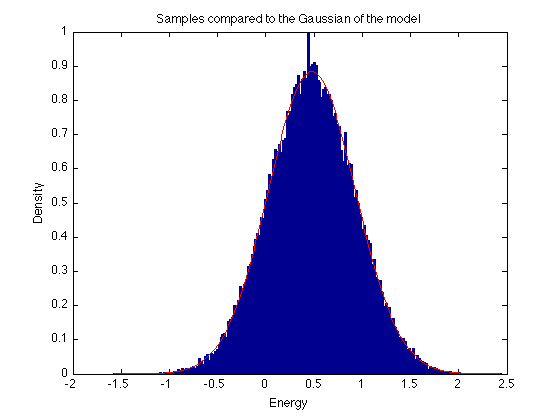
\includegraphics[width=0.5\textwidth]{figures/fig1.png}
\caption{Illustration of the samples drawn from the Gaussian part of the mixed distribution}
\label{label}
\end{figure}

% subsection test_of_sampling (end)

\subsection{Test of save/load date} % (fold)
\label{sub:test_of_save_load_date}

% subsection test_of_save_load_date (end)

% section testing_of_implementation (end)

\section{Results} % (fold)
\label{sec:results}
A presentation and discussion of the results obtained from its application to the protein dataset.
% section results (end)


\section{Conclusion} % (fold)
\label{sec:conclusion}

% section conclusion (end)

\section{Improvements} % (fold)
\label{sec:improvements}
The present implementation does not enable the user to specify which distributions should be part of the mixed node. Future work could involve making use of the existing distributions and using them in the mixed node. This would remove the duplicate code that is present in the current prototype of the mixed node, and make the mixed node more flexible.
% section improvements (end)

\bibliographystyle{abbrv}
\bibliography{bibliography}


\end{document}